\documentclass[12pt]{article}
\usepackage[polish]{babel}
\usepackage{float}
\usepackage{listings}
\usepackage[utf8]{inputenc}
\usepackage{amsmath}
\usepackage{pdfpages}
\usepackage[T1]{fontenc} % Add this line
    \title{Sprawozdanie z projektu 2, MOM}
    \author{Krzysztof Rudnicki, 307585}
    \date{\today}
\begin{document}
\maketitle
\section{Parametry}
z - stan początkowy \\
S - zakupione surowce (S = \{S1, S2\}) \\
G1 - surowiec S1 załadowany do wagonów \\
P - surowce w przygotowywalni (P = \{P1, P2\}) \\
O2 - surowiec S2 w zakładzie obróbki cieplnej \\
D - półprodukty (D = \{D1, D2\}) \\ 
W - wyroby (W = \{W1, W2\}) \\
N - stany surowców/półproduktów/wyrobów (zakupione surowce, surowce w przechowalni, surowce w zakładzie obróbki cieplnej, półprodukty, wyroby) \\ 
$r_w$ - cena sprzedaży wyrobu $w[\frac{1}{t}]$ \\
$u_{ij}$ - przepustowośc przepływu ze stanu i do stanu j[t] \\ 
$m_{pd}$ - mnożnik definiujący przepływ ze stanu 'surowiec w przygotowalni p' do stanu 'półprodukt d'

\section{Zmienne decyzyjne}
$f_{ij}$ = przepływ pomiędzy stanem i a stanem j [t] \\ 
\section{Zmienne pomocnicze}
$a_1$ - liczba zakupionego surowca S1 powyżej 2387 ton [t] \\
$a_2$ - liczba zakupionego surowca S1 powyżej 6659 ton [t] \\
$b_1$ - liczba zakupionego surowca S2 powyżej 2090 ton [t] \\
$b_2$ - liczba zakupionego surowca S2 powyżej 4349 ton [t] \\
$c_{P1}$ - liczba wagonów transportujących surowiec S1 do przygotowalni \\ 
$e_{P2}$ - liczba ciężarówek transportujących surowiec S2 do przygotowalni \\
$e_{O2}$ - liczba ciężarówek transportującyhc surowiec S2 do zakładu obróbki cieplnej \\
$g_1$ - zmienna binarna przyjmująca wartość 1 gdy przepływ ze stanu "zakupiony surowiec S2" (S2) do stanu "surowiec S2 w zakładzie obróbki cieplnej" (O2) jest większy niż 2000 ton i mniejszy niż 4000 ton \\ 
$g_2$ - zmienna binarna przyjmująca wartość 1 gdy przepływ ze stanu "zakupiony surowiec S2" (S2) do stanu "surowiec S2 w zakładzie obróbki cieplnej" (O2) jest większy niż 4000 ton i mniejszy niż 6000 ton \\
l - liczba pracowników zatrudnionych w przygotowalni
\section{Funkcja celu}
\begin{align*}
Q &= max[Zysk - Koszt] \\
&= max[\sum_{i \in N, w \in W} r_w + f_{iw} \\
&- (19f_{zS1} - 5a_1 - 4a_2 + 11f_{zS2} + 2b_1 + 2b_2 \\
&+ 1290c_{P1} + 1500e_{P2} +1500e_{O2} + 160l + 10000g_1 + 40000g_2)] 
\end{align*}

\section{Ograniczenia}
\subsection{Ogólne}
Przepływ musi być nieujemny oraz mniejszy przepustowości
\begin{equation}
0 \leq f_{ij} \leq u_{ij}, \qquad (i,j) \in N \\
\end{equation}
Wszystko co przypłyneło do stanu k musi stamtąd "odpłynąć"
\begin{equation}
\sum_{i \in N \backslash \{z\}} f_{ki} = \sum_{i \in N \backslash \{W\}} f_{jk}, \qquad k \in N \backslash \{z, W\}
\end{equation}

\subsection{Dostępne surowce}
Nie możemy kupić więcej surowca S1 niż jest dostępne
\begin{equation}
f_{zS1} \leq 12000
\end{equation}
Nie możemy kupić więcej surowca S2 niż jest dostępne
\begin{equation}
f_{zS2} \leq 8000
\end{equation}

\subsection{Koszt zakupu surowców}
Nie możemy kupić mniej niż 0 surowców
\begin{equation}
a_1 \geq 0
\end{equation}
\begin{equation}
a_2 \geq 0
\end{equation}
\begin{equation}
b_1 \geq 0
\end{equation}
\begin{equation}
b_2 \geq 0
\end{equation}
Ograniczamy ile ton ponad dany limit kupiliśmy
\begin{equation}
a_1 \leq f_{zS1} - 2387
\end{equation}
liczba powyżej 2056 ton
\begin{equation}
a_2 \leq f_{zS1} - 6659
\end{equation}
liczba powyżej 2056 ton
\begin{equation}
b_1 \leq f_{zS2} - 2090
\end{equation}
liczba powyżej 2056 ton
\begin{equation}
b_2 \leq f_{zS2} - 4349
\end{equation}
\subsection{Transport surowca S1 do przygotowalni}
wagon może przetransportować maks. 18 ton surowca S1
\begin{equation}
b_{P1} \geq [\frac{ f_{S1, G1} }{18}]
\end{equation}
\subsection{Transport surowca S2 do przygtowalni}
ciężarówka może przetransportować maks. 25 ton surowca S2
\begin{equation}
c_{P2} \geq [ \frac{ f_{S2, P2} }{ 25 } ]
\end{equation}
\subsection{Praca przygotowalni}
Przygotowalnia nie może mieć więcej surowców niż przepustowości
\begin{equation}
\sum_{i \in N, p \in P} f_{ip} \leq 16000
\end{equation}
ilość półproduktów w zależności od surowca
\begin{equation}
(\sum_{i \in N} f_{ip}) m_{pd} = f_{pd}, \qquad i \in N, p \in P, d \in D
\end{equation}
\subsection{Koszt pracy przygotowalni}
3 pracowników może obsługiwać maksymalnie 150 ton całkowitej ilości przerabianych surowców
\begin{equation}
l \geq [ \frac{ \sum_{i\in N, p \in P} f_{ip} }{150} ]
\end{equation}
\subsection{Transport S2 do zakładu obróbki cieplnej}
ciężarówka może przetransportować maks. 25 ton surowca S2
\begin{equation}
c_{O2} \geq [\frac{ f_{S2, O2} }{25}]
\end{equation}
\subsection{Praca zakładu obróbki cieplnej}
ilość surowca S2 w zakładzie obróbki cieplnej nie może być większa od 6000
\begin{equation}
f_{S2, O2} \leq 6000
\end{equation}
\subsection{Minimalna dostarczona ilość wyrobów}
Zgodnie z umową musimy dostarczyć przynajmniej 5000 ton wyrobów
\begin{equation}
\sum_{i \in N f_{iw}} \geq 5000, \qquad w \in W
\end{equation}
\subsection{Maksymalna liczba wagonow}
Na jedna lokomotywę, nie może przypadać więcej niż 12 wagonów
\begin{equation}
12wl \geq c_{P1}
\end{equation}

\section{Model sieciowy}
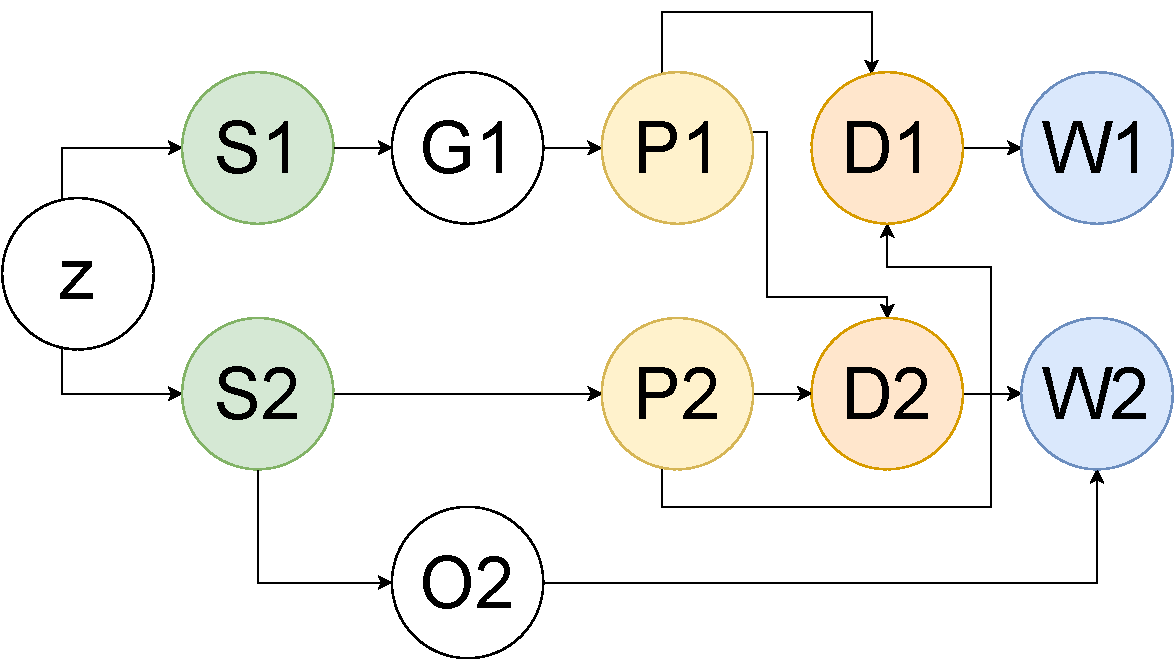
\includepdf{mom2.drawio.pdf}

\section{Implementacja modelu}
\begin{lstlisting}[caption= plik mod]
# PARAMETRY
# Stan poczatkowy
set Z;
# Zakupione surowce, s1 i s2
set S; set S1; set S2;
# Surowiec S1 zaladowany do wagonow
set G1;
# Surowce w przygotowywalni
set P; set P1; set P2;
# Surowiec S2 w zakladzie obrobki cieplnej
set O2;
# Polprodukty 
set D; set D1; set D2;
# Wyroby
set W; set W1; set W2;
# Stany surowcow, zakupione, wyroby, obrobka cieplna
set N; set Nz; set Nw; set Nzw;

# Cena sprzedazy wyrobu
param r{w in W};
# Przepustowosc przeplwyu z jednego stanu do drugiego
param u{i in N, j in N};
# Mnoznik definijujacy przepwy ze stanu surowiec
# w przygotowalni do stanu polprodukt
param m{p in P, d in D};

# ZMIENNE DECYZYJNE
# przeplyw pomiedzy stanem i a stanem j
var f{i in N, j in N}, >= 0, integer; # Ograniczenie 1

# Zmienne pomocnicze
# liczba zakupionego surowca S1 powyzej 2387 ton
var a1, >= 0, integer; # Ograniczenie 5
# liczba zakupionego surowca S1 powyzej 6659 ton
var a2, >= 0, integer; # Ograniczenie 6
# liczba zakupionego surowca S2 powyzej 2090 ton
var b1, >= 0, integer; # Ograniczenie 7
# liczba zakupionego surowca S2 powyzej 4349 ton
var b2, >= 0, integer; # Ograniczenie 8
# liczba wynajetych lokomotyw
var wl, >= 0, integer;
# liczba wagonow transportujacych surowiec S1 do przygotowalni
var cp1, >= 0, integer;
# liczba ciezarowek transportujacych surowiec S2 do przygotowalni
var ep2, >= 0, integer; 
# liczba ciezarowek transportujacych surowiec S2
# do zakladu obrobki cieplnej
var eo2, >= 0, integer;
var e1, >= 0, <=1, integer;
var e2, >= 0, <=1, integer;
# Liczba pracownikow
var l, >= 0, integer;

maximize Q: (sum {i in N, w in W} r[w] * f[i,w])
- (19* (sum {z in Z, s1 in S1} f[z, s1] )
- 5*a1 
- 4*a2 
+ 11*  sum {z in Z, s2 in S2} (f[z, s2])
+ 2*b1 
+ 2*b2
+ 1290*cp1
+ 1500*ep2 
+ 1500*eo2 
+ 160*l 
+ 10000*e1 
+ 40000*e2);

# OGRANICZENIA
subject to
  # Ogolne i Dostepne surowce
  Ogr_1_3_4{i in N, j in N}:
    f[i,j] <= u[i,j];
  Ogr_2{k in Nzw}:
    sum {i in Nz} f[k,i] = sum {j in Nw} f[j,k];    
  # Koszt zakupu surowcow
  Ogr_9{z in Z, s1 in S1}:
    a1 <= f[z,s1] - 2387;
  Ogr_10{z in Z, s1 in S1}:
    a2 <= f[z,s1] - 6659;
  Ogr_11{z in Z, s2 in S2}:
    b1 >= f[z,s2] - 2090;
  Ogr_l2{z in Z, s2 in S2}:
    b2 >= f[z,s2] - 4349;
  # Transport surowca S1
  Ogr_13{s1 in S1, g1 in G1}:
   cp1 >= f[s1,g1] / 18;
  # Transport surowca S2
  Ogr_14{s2 in S2, p2 in P2}:
    ep2 >= f[s2,p2] / 25;
  # Praca przygotowalni
  Ogr_15: 
    sum {i in N, p in P} f[i,p] <= 16000;
  Ogr_16{p in P, d in D}:
    (sum {i in N} f[i,p]) * m[p,d] = f[p,d];
  # Koszt pracy przygotowalni
  Ogr_17: 
    l >= (sum {i in N, p in P} f[i,p])/150;
  # Transprot S2 do obrobki cieplnej
  Ogr_18{s2 in S2, o2 in O2}:
    eo2 >= f[s2,o2] / 25;
  # Praca zakladu obrobki cieplnej
  Ogr_19{s2 in S2, o2 in O2}:
    f[s2,o2] <= 6000;
  # Minimalna dostarczona ilosc wyrobow
  Ogr_20{w in W}:
   	sum {i in N} f[i,w] >= 5000;
  # Na jedna lokomotywe przypada co najwyzej 12 wagonow
  Ogr_21:
   12 * wl >= cp1;
  
solve;
display {i in N, j in N: f[i,j] > 0}: f[i,j];
display: a1; display: a2; display: b1; display: b2; display: wl;
display: cp1; display: ep2; display: eo2; display: 
e1; display: l;
\end{lstlisting}

\begin{lstlisting}[caption= plik dat]
data;
set Z := z;
set S := s1, s2;
set S1 := s1;
set S2 := s2;
set G1 := g1;
set P := p1, p2;
set P2 := p2;
set O2 := o2;
set D := d1, d2;
set W := w1, w2;
set N := z, s1, s2, g1, p1, p2, o2, d1, d2, w1, w2;
set Nz := s1, s2, g1, p1, p2, o2, d1, d2, w1, w2;
set Nw := z, s1, s2, g1, p1, p2, o2, d1, d2;
set Nzw := s1, s2, g1, p1, p2, o2, d1, d2;
param r := w1 467 w2 480;
param u := 
z  z     0  z s1  12000  z s2  8000  z g1     0  z p1     0 
z p2     0  z o2     0  z d1     0  z d2     0  z w1     0  z w2     0 
s1  z     0 s1 s1     0 s1 s2     0 s1 g1 99999 s1 p1     0 
s1 p2     0 s1 o2     0 s1 d1     0 s1 d2     0 s1 w1     0 s1 w2     0 
s2  z     0 s2 s1     0 s2 s2     0 s2 g1     0 s2 p1     0 
s2 p2 99999 s2 o2 99999 s2 d1     0 s2 d2     0 s2 w1     0 s2 w2     0 
g1  z     0 g1 s1     0 g1 s2     0 g1 g1     0 g1 p1 99999 
g1 p2     0 g1 o2     0 g1 d1     0 g1 d2     0 g1 w1     0 g1 w2     0 
p1  z     0 p1 s1     0 p1 s2     0 p1 g1     0 p1 p1     0 
p1 p2     0 p1 o2     0 p1 d1 99999 p1 d2 99999 p1 w1     0 p1 w2     0 
p2  z     0 p2 s1     0 p2 s2     0 p2 g1     0 p2 p1     0 
p2 p2     0 p2 o2     0 p2 d1 99999 p2 d2 99999 p2 w1     0 p2 w2     0 
o2  z     0 o2 s1     0 o2 s2     0 o2 g1     0 o2 p1     0 
o2 p2     0 o2 o2     0 o2 d1     0 o2 d2     0 o2 w1     0 o2 w2 99999 
d1  z     0 d1 s1     0 d1 s2     0 d1 g1     0 d1 p1     0 
d1 p2     0 d1 o2     0 d1 d1     0 d1 d2     0 d1 w1 99999 d1 w2     0 
d2  z     0 d2 s1     0 d2 s2     0 d2 g1     0 d2 p1     0 
d2 p2     0 d2 o2     0 d2 d1     0 d2 d2     0 d2 w1     0 d2 w2 99999 
w1  z     0 w1 s1     0 w1 s2     0 w1 g1     0 w1 p1     0 
w1 p2     0 w1 o2     0 w1 d1     0 w1 d2     0 w1 w1     0 w1 w2     0 
w2  z     0 w2 s1     0 w2 s2     0 w2 g1     0 w2 p1     0 
w2 p2     0 w2 o2     0 w2 d1     0 w2 d2     0 w2 w1     0 w2 w2     0;
param m := p1 d1 0.1 p1 d2 0.9 p2 d1 0.1 p2 d2 0.9;
end;
\end{lstlisting}

\section{Wyniki}
Model z takimi ograniczeniami \textbf{nie znajduje} rozwiązania \\
Problemem jest tu ogranicznie mówiące o tym że należy dostaczyć co najmniej \textbf{5000} ton \textbf{każdego} produktu \\
To ograniczenie jest niewykonywalne gdyż nawet zakładając dostarczenie maksymalnej liczby ton surowców (12000 + 8000 = 20000) ton, i ignorując ograniczenie przepustowośći przygotowalni 16000 ton, nie jesteśmy w stanie wytworzyć wystarczająco półproduktu D1 aby wytworzyć wystarczająco wyrobu W1 \\ 
gdybyśmy całość dostępnych surowców (znowu, ignorując przepustowość przygotowalni), zużyli na wytwarzanie tylko i wyłącznie półproduktu D1 z którego potem uzyskujemy wyrób W1, otrzymalibyśmy: 
\[ (12000 + 8000) * 0.1 = 20000 * 0.1 = 2000 \]
maksymalna liczba ton wyrobu W1 którą możemy uzyskać, ignorując przepustowość przygotowywalni oraz wymagania dotyczące W2 wynosi 2000 ton, czyli mniej niż 5000 wymaganych ton \\
W związku z tym wyniki przedstawione niżej dotyczącą przypadku w którym \textbf{ignorujemy} ograniczenie związane z minimalną liczbą ton każdego produktu który musimy dostarczyć (ograniczenie 20) \\
\begin{figure}[H]
\caption{}
\begin{tabular}{|c|c|c|c|c|c|c|c|c|c|c|c|}
\hline
 & 	z & S1 & S2 & G1 & P1 & P2 & O2 & D1 & D2 & W1 & W2 \\
\hline
z &	0 & 12000 & 8000 & 0 & 0 & 0 & 0 & 0 & 0 & 0 & 0 \\
\hline
S1 &	0 & 0 & 0 & 12000 & 0 & 0 & 0 & 0 & 0 & 0 & 0 \\
\hline
S2 &	0 & 0 & 0 & 0 & 0 & 2000 & 6000 & 0 & 0 & 0 & 0 \\
\hline
G1 &	0 & 0 & 0 & 0 & 12000 & 0 & 0 & 0 & 0 & 0 & 0 \\
\hline
P1 &	0 & 0 & 0 & 0 & 0 & 0 & 0 & 1200 & 10800 & 0 & 0 \\
\hline
P2 &	0 & 0 & 0 & 0 & 0 & 0 & 0 & 200 & 1800 & 0 & 0 \\
\hline
O2 &	0 & 0 & 0 & 0 & 0 & 0 & 0 & 0 & 0 & 0 & 6000 \\
\hline
D1 &	0 & 0 & 0 & 0 & 0 & 0 & 0 & 0 & 0 & 1400 & 0 \\
\hline
D2 &	0 & 0 & 0 & 0 & 0 & 0 & 0 & 0 & 0 & 0 & 12600 \\
\hline
W1 &	0 & 0 & 0 & 0 & 0 & 0 & 0 & 0 & 0 & 0 & 0 \\
\hline
W2 &	0 & 0 & 0 & 0 & 0 & 0 & 0 & 0 & 0 & 0 & 0 \\
\hline

\end{tabular}
\end{figure}

\[ a_1 = 9613 \]
\[ a_2 = 5341 \]
\[ b_1 = 5910 \]
\[ b_2 = 3651 \]
\[ w_1 = 56 \]
\[ c_{P1} = 667 \]
\[ e_{P2} = 80 \]
\[ e_{O2} = 240 \]
\[ e_1 = 0 \]
\[ e_2 = 0 \]
\[ l = 94 \]
Ponownie, wyniki powyżej są prawdziwe wyłącznie dla przypadku w którym \textbf{ignorujemy ograniczenie numer 20}

\end{document}